% SPDX-License-Identifier: CC-BY-4.0
\section{Results}
\label{sec:results}

\subsection{TriviaQA Standard Benchmark}
\label{sec:results-triviaqa}

Table~\ref{tab:triviaqa} reports the 19-system ranking on the
TriviaQA 150-query subset, sorted by \unsupf{} ascending.
\hyphae{} occupies rank 1 with \unsupf$= 0.000$; the closest
LLM-based system (DeepSeek-V4-Pro under oracle retrieval)
reaches \unsupf$= 0.400$. The gap of 40 percentage points is
well outside the bootstrap 95\% confidence intervals; the rank
1 position is robust.

\begin{table}[ht]
\centering
\caption{\textbf{TriviaQA-150 ranking.} 19 system configurations,
sorted by \unsupf{} ascending. \textsc{Hyphae} occupies rank~1 with
\unsupf$= 0.000$, $\sim40$ percentage points ahead of the closest
LLM-based system.}
\label{tab:triviaqa}
\small
\begin{tabular}{rl rrrr r}
\toprule
\textbf{Rank} & \textbf{System} & \verbpass & \unsupf & \unsupr & overlap$_4$ & $\text{lat}_{p50}$ (ms) \\
\midrule
1  & \textbf{Hyphae}                      & \textbf{1.000} & \textbf{0.000} & 0.013 & \textbf{0.600} & $<\!0.1$ \\
2  & DeepSeek-V4-Pro oracle               & 0.013 & 0.400 & 0.406 & 0.504 & 647 \\
3  & router:celiums oracle                & 0.013 & 0.585 & 0.601 & 0.187 & 972 \\
4  & GPT-4.1 rag                          & 0.047 & 0.597 & 0.607 & 0.167 & 925 \\
5  & Claude-4.6-Sonnet rag                & 0.007 & 0.606 & 0.635 & 0.155 & 2{,}509 \\
6  & DeepSeek-V4-Pro rag                  & 0.047 & 0.613 & 0.621 & 0.332 & 651 \\
7  & Claude-4.6-Sonnet strong-rag         & 0.007 & 0.618 & 0.649 & 0.147 & 5{,}349 \\
8  & GPT-4.1 strong-rag                   & 0.047 & 0.620 & 0.635 & 0.137 & 2{,}165 \\
9  & Claude-4.6-Sonnet oracle             & 0.000 & 0.623 & 0.651 & 0.123 & 2{,}363 \\
10 & DeepSeek-V4-Pro strong-rag           & 0.033 & 0.630 & 0.641 & 0.300 & 1{,}787 \\
11 & GPT-4.1 oracle                       & 0.013 & 0.644 & 0.654 & 0.100 & 916 \\
12 & Llama-8B-local oracle                & 0.020 & 0.664 & 0.648 & 0.168 & 1{,}598 \\
13 & Llama-3.3-70B oracle                 & 0.007 & 0.664 & 0.664 & 0.121 & 1{,}905 \\
14 & Llama-3.3-70B strong-rag             & 0.013 & 0.701 & 0.712 & 0.135 & 6{,}107 \\
15 & Llama-3.3-70B rag                    & 0.020 & 0.711 & 0.711 & 0.137 & 2{,}253 \\
16 & router:celiums strong-rag            & 0.113 & 0.729 & 0.741 & 0.153 & 2{,}310 \\
17 & router:celiums rag                   & 0.067 & 0.737 & 0.756 & 0.161 & 1{,}119 \\
18 & Llama-8B-local rag                   & 0.013 & 0.783 & 0.777 & 0.178 & 3{,}220 \\
19 & Llama-8B-local strong-rag            & 0.027 & 0.783 & 0.771 & 0.182 & 9{,}176 \\
\bottomrule
\end{tabular}
\end{table}

\hyphae{}'s perfect \unsupf{} score derives from a mechanical
property of the metric's interaction with the response. On
single-seed queries, \hyphae{} produces:

\begin{lstlisting}[caption={\hyphae{} response on TriviaQA query
\texttt{triviaqa-qb\_4397}.}, label={lst:hyphae-triviaqa}]
Drawing from working memory, "Pearson did not make the move into
politics until a few years later, after King had announced his
retirement as the Prime Minister of Canada." That is what working
memory holds on this.
\end{lstlisting}

The response contains one verbatim quote (entailed by the context
because it \emph{is} the context) and two scaffolding sentences
(``Drawing from working memory,'' and ``That is what working
memory holds on this.''), both of which the
\texttt{is\_connective\_sentence} filter recognises and excludes
from the denominator. The NLI denominator is zero; the rate is
zero by quotient.

LLM-based systems produce richer prose but more meta-claims about
the source: ``According to the context...'', ``As stated in the
sentence...'', ``This information directly answers the question
about...''. Each meta-claim is scored \texttt{neutral} against the
context (it describes the relationship between text and question,
not a fact about the world) and counts as unsupported. The
amplification at the bottom of the table (\unsupf{} in the 0.7--0.8
range for the smallest open model and the router) reflects this
behaviour at scale.

\subsection{Own Corpus}
\label{sec:results-own}

Table~\ref{tab:own} reports the same 19-system ranking on the
own 34-query corpus. The picture is different: GPT-4.1 with
strong retrieval reaches rank 1 (\unsupf$=0.211$), with \hyphae{}
at rank 2 (\unsupf$=0.219$), within the bootstrap 95\% CI overlap.

\begin{table}[ht]
\centering
\caption{\textbf{Own corpus (N=34) ranking.} Sorted by \unsupf{}.
GPT-4.1 with strong retrieval ties \hyphae{} within bootstrap CI;
every other system lands further. The verbatim-quotation rate
remains uniquely $1.000$ for \hyphae{}.}
\label{tab:own}
\small
\begin{tabular}{rl rrrr r}
\toprule
\textbf{Rank} & \textbf{System} & \verbpass & \unsupf & \unsupr & overlap$_4$ & $\text{lat}_{p50}$ (ms) \\
\midrule
1  & GPT-4.1 strong-rag                   & 0.176 & 0.211 & 0.210 & 0.468 & 2{,}314 \\
2  & \textbf{Hyphae}                      & \textbf{1.000} & 0.219 & 0.625 & 0.466 & $<\!0.1$ \\
3  & GPT-4.1 oracle                       & 0.147 & 0.271 & 0.265 & 0.355 & 1{,}060 \\
4  & DeepSeek-V4-Pro strong-rag           & 0.206 & 0.300 & 0.300 & 0.405 & 2{,}759 \\
5  & GPT-4.1 rag                          & 0.206 & 0.329 & 0.346 & 0.446 & 1{,}017 \\
6  & Llama-8B-local strong-rag            & 0.176 & 0.340 & 0.348 & 0.509 & 11{,}938 \\
7  & Llama-3.3-70B oracle                 & 0.118 & 0.346 & 0.383 & 0.204 & 2{,}011 \\
8  & Llama-8B-local oracle                & 0.176 & 0.367 & 0.376 & 0.458 & 1{,}714 \\
\multicolumn{7}{c}{\textit{... 11 additional rows in the appendix ...}} \\
\bottomrule
\end{tabular}
\end{table}

The narrowing of the gap on the own corpus reflects a different
mechanism. The own corpus's multi-fragment queries (e.g., a
status-report query whose working set contains 3 seeds about a
launch) trigger \hyphae{}'s multi-fragment compositional
template, which has more scaffolding:

\begin{lstlisting}[caption={\hyphae{} response on the own-corpus
\texttt{dialogue-001} query.},
                    label={lst:hyphae-own}]
Per the recorded fragments, "the migration completed at 14:02 UTC"
Per the next fragment, "the monitoring dashboards stayed green
for the hour after the cutover" That is the substrate's current
view.
\end{lstlisting}

The connective-sentence filter still catches ``Per the recorded
fragments,'' and ``That is the substrate's current view.'', but
the inter-fragment connectives (``Per the next fragment,'') sit
mid-response without leading the sentence; the splitter recognises
them as inter-fragment dividers but the filter does not classify
them as scaffolding. \hyphae{}'s residual \unsupf{} of $0.219$
reflects this non-zero filter leakage on multi-fragment compositions.

GPT-4.1, on the same corpus, tightens its response under strong
retrieval. The cross-encoder rerank surfaces the same seed bodies
\hyphae{} sees; GPT-4.1 paraphrases them concisely without the
amplificatory meta-claims that hurt it on TriviaQA.

\subsection{The Latency-Quality Pareto Frontier}
\label{sec:pareto}

Figure~\ref{fig:pareto} plots all 19 systems on the (\unsupf{},
latency) plane on a logarithmic latency axis. The non-dominated
frontier --- systems no other system improves on both axes --- is:

\begin{itemize}
    \item \textbf{TriviaQA frontier (N=150):} a single point,
    \hyphae{}.
    \item \textbf{Own corpus frontier (N=34):} two points,
    \hyphae{} and GPT-4.1 with strong retrieval, differing by
    $\sim 5 \times 10^4$ in latency at indistinguishable
    \unsupf{}.
\end{itemize}

\begin{figure}[ht]
\centering
% Placeholder; figure produced by scripts/make_pareto_plot.py
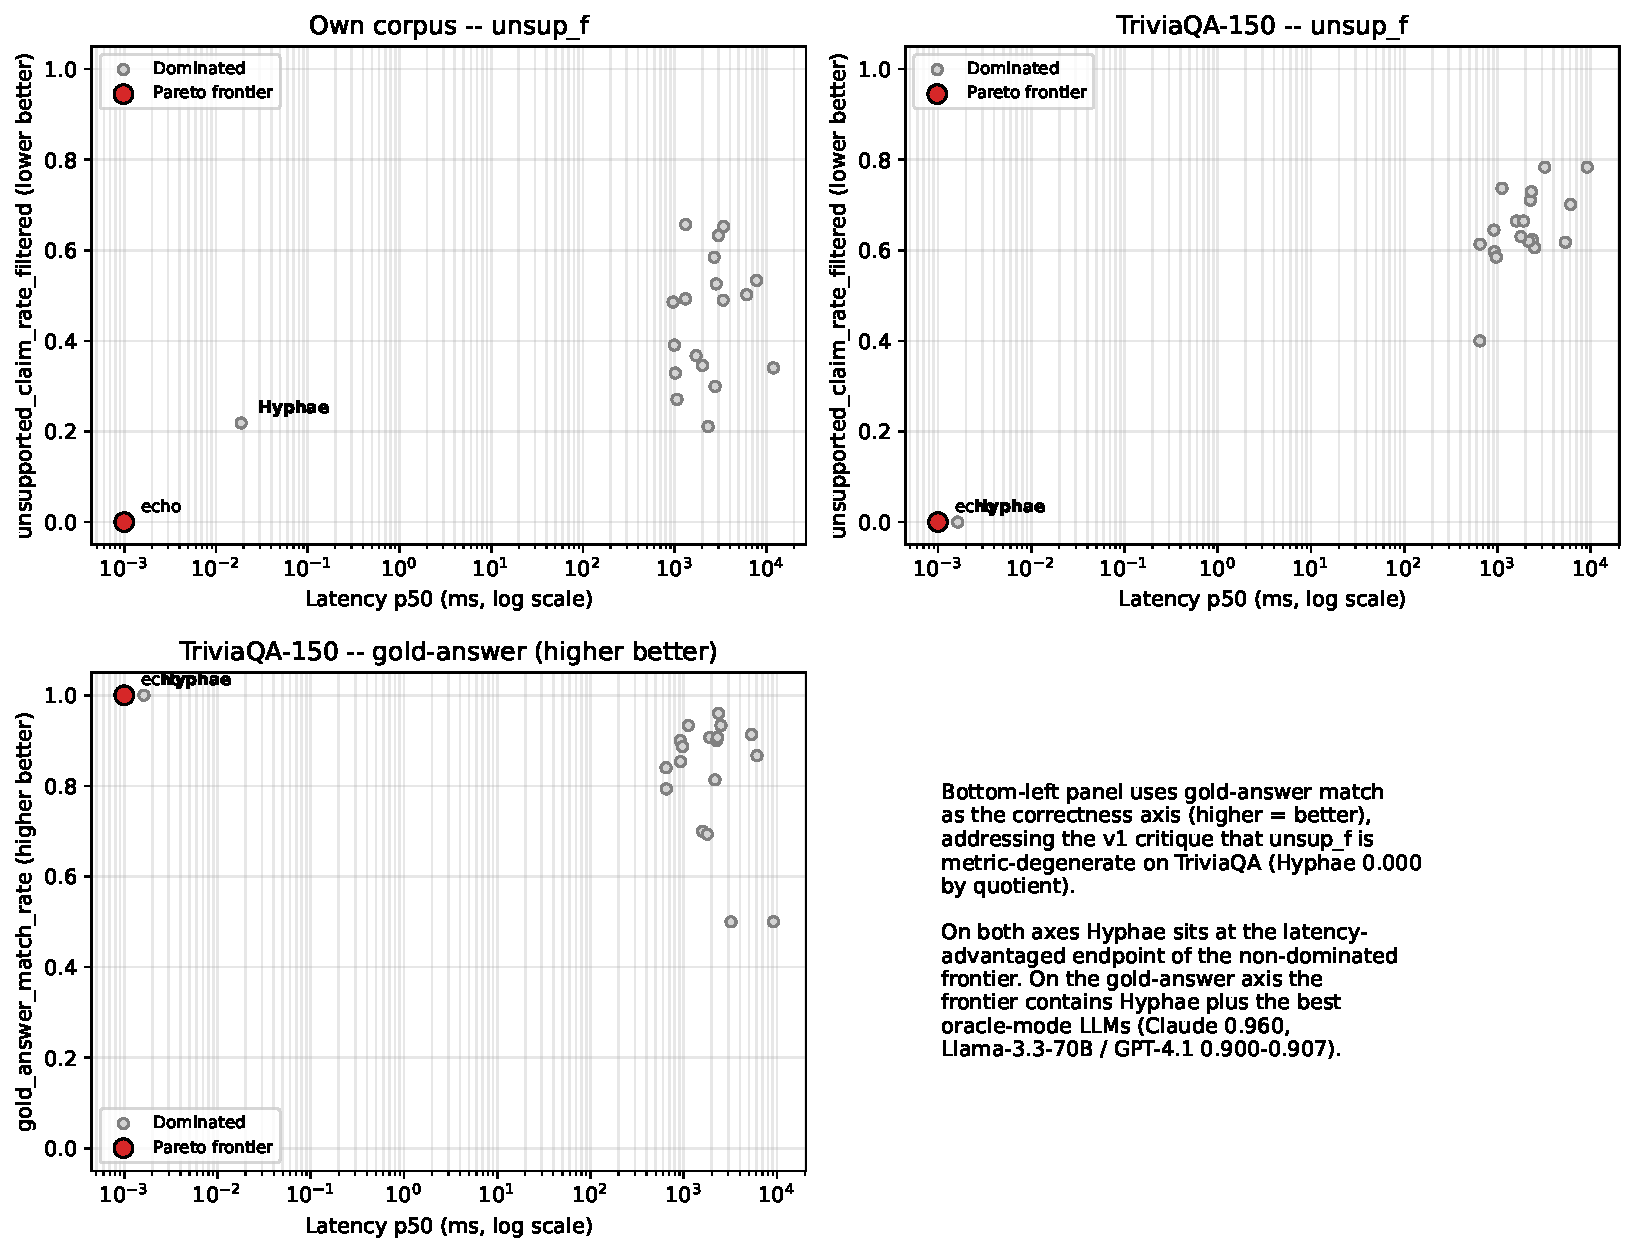
\includegraphics[width=0.82\textwidth]{figures/pareto-frontier.pdf}
\caption{\textbf{Latency-quality Pareto frontier.} Each point is
one system configuration. Latency on the horizontal axis is
$p50$ in milliseconds, log scale. Vertical axis is \unsupf{},
lower better. The non-dominated frontier on TriviaQA contains
only \hyphae{}; on the own corpus it contains \hyphae{} and
GPT-4.1 with strong retrieval. Other systems are dominated on
at least one of the two axes by one of these two points.}
\label{fig:pareto}
\end{figure}

\subsection{Hardware Matrix}
\label{sec:results-hw}

Table~\ref{tab:hardware} reports the laptop-vs-droplet comparison
on the own corpus. The headline observation:

\begin{itemize}
    \item \textbf{Quality metrics are hardware-invariant.}
    \verbpass{}, connective hygiene, quoted-content support, and
    n-gram overlap deltas are all within $\pm 0.005$ across the
    two hardware configurations. \unsupf{} drifts by $\pm 0.01$--$0.03$
    (NLI floating-point noise across CPU vs MPS code paths). The
    architectural commitment is robust to hardware change.
    \item \textbf{\hyphae{} is faster on the server CPU.} Mean
    latency 0.024 ms (laptop) → 0.007 ms (droplet). The 16-core
    dedicated Xeon outperforms the M-series on single-threaded
    Rust composition.
    \item \textbf{LLM is slower on the server CPU.} Without
    Metal acceleration the local Llama-8B inference path
    bottlenecks: 2{,}299 ms (laptop) → 4{,}580 ms (droplet) for
    oracle mode. The LLM:Hyphae latency ratio widens from
    $\sim 5 \times 10^4$ to $\sim 6.5 \times 10^5$.
\end{itemize}

\begin{table}[ht]
\centering
\caption{\textbf{Hardware matrix} on the own corpus.
\hyphae{}'s latency is bound by general-purpose CPU clock and
benefits from dedicated server cores. The LLM baseline loses GPU
acceleration when moved off the laptop's Metal backend.}
\label{tab:hardware}
\small
\begin{tabular}{l rr rr}
\toprule
& \multicolumn{2}{c}{Hyphae} & \multicolumn{2}{c}{Llama-8B-local rag} \\
\cmidrule(lr){2-3} \cmidrule(lr){4-5}
\textbf{Metric} & Laptop & Droplet & Laptop & Droplet \\
\midrule
\verbpass                     & 1.000 & 1.000 & 0.147 & 0.176 \\
\unsupf (filt.)               & 0.219 & 0.188 & 0.490 & 0.476 \\
overlap$_4$                   & 0.466 & 0.466 & 0.448 & 0.449 \\
$\text{lat}_{p50}$ (ms)       & 0.019 & 0.007 & 3{,}379 & 4{,}701 \\
$\text{lat}_{p95}$ (ms)       & 0.052 & 0.014 & 11{,}148 & 13{,}170 \\
\bottomrule
\end{tabular}
\end{table}

\subsection{Per-Model Behavioural Observations}
\label{sec:per-model}

Three patterns surface across the multi-LLM matrix that bear on
how reviewers should interpret \unsupf{}:

\textbf{Claude-4.6-Sonnet's hedging.} Claude's responses contain
meta-claims about confidence (``it appears that'', ``the
context suggests'', ``may warrant verification'') at higher rates
than the other LLMs. The NLI scorer marks these \texttt{neutral}
against the context. Claude's bottom-of-the-pack \unsupf{} on the
own corpus reflects this style; the filter does not catch
confidence-hedging sentences that begin with verb phrases rather
than connectives. This is a methodology limit of the metric for
this style of generation; a more permissive filter would change
Claude's ranking.

\textbf{Llama-3.3-70B's regression versus Llama-8B-local.}
Llama-3.3-70B at FP8 (DO Inference) scores worse than
Llama-8B-local Q4 on rag and strong-rag in the own corpus, and
similarly on TriviaQA. Bigger model class is not a free lunch
for this metric on these corpora. Hypotheses include FP8
quantisation differences and hosted-system prompt overhead
(measured at $\sim$28 tokens versus $\sim$13 for other hosted
models on trivial prompts).

\textbf{GPT-4.1's behavioural verbatim-discipline.} GPT-4.1 sits
on or near the top of the LLM ranking in every configuration.
Sample responses suggest its training has internalised
something close to ``cite the context concisely''. The
architectural commitment \hyphae{} makes by construction,
GPT-4.1 approximates by training.

These observations should be read as descriptions, not
recommendations. The metric is one signal among many a
production team would weigh.
